\documentclass[tikz,border=10pt]{standalone}
\usetikzlibrary{positioning}
\usepackage{tkz-graph}
\usepackage{rotating}
\usetikzlibrary{arrows}
\usetikzlibrary{arrows.meta}

\begin{document}

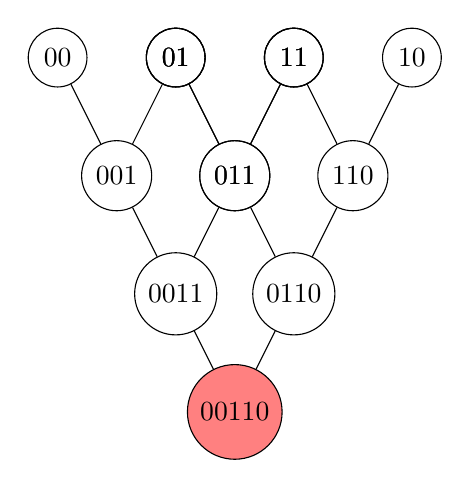
\begin{tikzpicture}[rotate=180]
\tikzstyle{every node}=[draw,circle]
\node[fill=red!50] {00110}
    child {node {0110}
        child {node {110}
            child{node {10}}
            child{node {11}}
        }
        child {node {011}
            child{node {11}}
            child{node {01}}
        } 
    }
    child {node {0011}
        child {node {011}
            child{node {11}}
            child{node {01}}
            }
        child {node {001}
            child{node {01}}
            child{node {00}}
            }
    };
\end{tikzpicture}

\end{document}